\textbf{Ejemplo 3}\\

Supongamos que hay en estudio dos opciones de inversión: el proyecto A que requiere una inversión inicial de  COP  200.000 y produce un ingreso de  COP  31.160 durante 10 períodos y el proyecto B que tiene un costo de  COP  100.000 y produce un ingreso durante 10 períodos de  COP  16.280. Con una tasa de oportunidad del 5\% período mes vencido determinar cuál es el mejor proyecto
\\

\textbf{Solución.}\\
%La tabla ira centrada
\begin{center}
	\renewcommand{\arraystretch}{1.5}% Margenes de las celdas
	%Creación de la cuadricula de 3 columnas
\begin{longtable}[H]{|c|c|c|}
		%Creamos una linea horizontal
\hline
		%Definimos el color de la primera fila
\rowcolor[HTML]{FFB183}
%%%%% INICIO ASIGNACIÓN PERÍODO FOCAL %%%%%%%
  %%%%%%%%%% INICIO TITULO
  %Lo que se hace aquí es mezclar las 3 columnas en una sola
  \multicolumn{3}{|c|}{\cellcolor[HTML]{FFB183}\textbf{1. Asignación período focal}}   \\ \hline
  %%%%%%%%%% FIN TITULO
  %%%%% INICIO DECLARACIÓN DE VARIABLES %%%%%%%
  \multicolumn{3}{|c|}{$pf = 0 pmv$}   \\ \hline

%%%%%%%%%%% INICIO TITULO
\rowcolor[HTML]{FFB183}
\multicolumn{3}{|c|}{\cellcolor[HTML]{FFB183}\textbf{2. Declaración de variables}}    \\ \hline
%%%%%%%%%%% FIN TITULO
%%%%%%%%%%% INICIO MATEMÁTICAS

$\textbf{Proyecto A}$                                     & \multicolumn{2}{c|}{$ \textbf{Proyecto B} $} \\
$i = 5\% pmv = TIO \hspace{0.3cm} $	& \multicolumn{2}{c|}{$ i = 5\% pmv = TIO $} \\
$ n = 10 pmv $	&	\multicolumn{2}{c|}{ $ n = 10 pmv $ } \\
$\text{Inversión inicial} =  COP  200.000 $	&	\multicolumn{2}{c|}{ $ \text{Inversión inicial} =  COP  100.000$ } \\ 
$ \text{Ingreso por 10 periodos} =  COP  31.160 $	&	\multicolumn{2}{c|}{ $ \text{Ingreso por 10 periodos} =  COP  16.280 $ }
\\
$  $	&	\multicolumn{2}{c|}{ $ $ }
\\
\hline
%%%%%%%%%% FIN MATEMÁTICAS
		%%%%% INICIO FLUJO DE CAJA
\rowcolor[HTML]{FFB183}
\multicolumn{3}{|c|}{\cellcolor[HTML]{FFB183}\textbf{3. Diagrama de flujo de caja}} \\ \hline
		%Mezclamos 3 columnas y pondremos el dibujo
		%%%%%%%%%%%%% INSERCIÓN DE LA IMAGEN
		%Deberán descargar las imágenes respectivas del drive y pegarlas en la carpeta
		%n_capitulo/img/ejemplos/1/capitulo1ejemplo1.pdf  (el /1/ es el numero del ejemplo)
\multicolumn{3}{|c|}{ 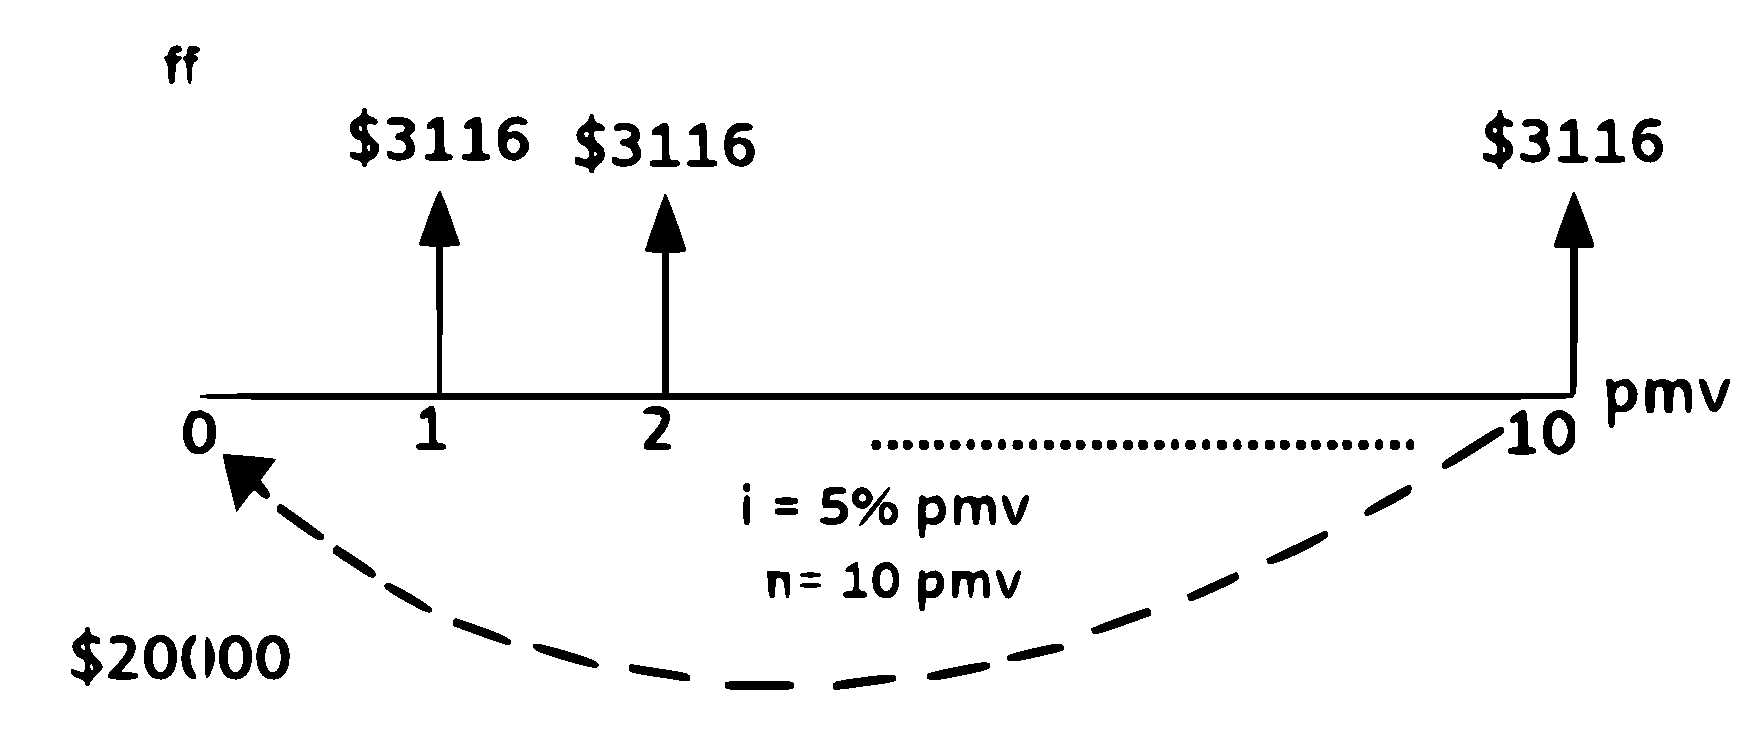
\includegraphics[scale=0.4, trim=-5 -5 -5 -5]{Graf8Cap11.pdf} }   
   \\ 
\multicolumn{3}{|c|}{ 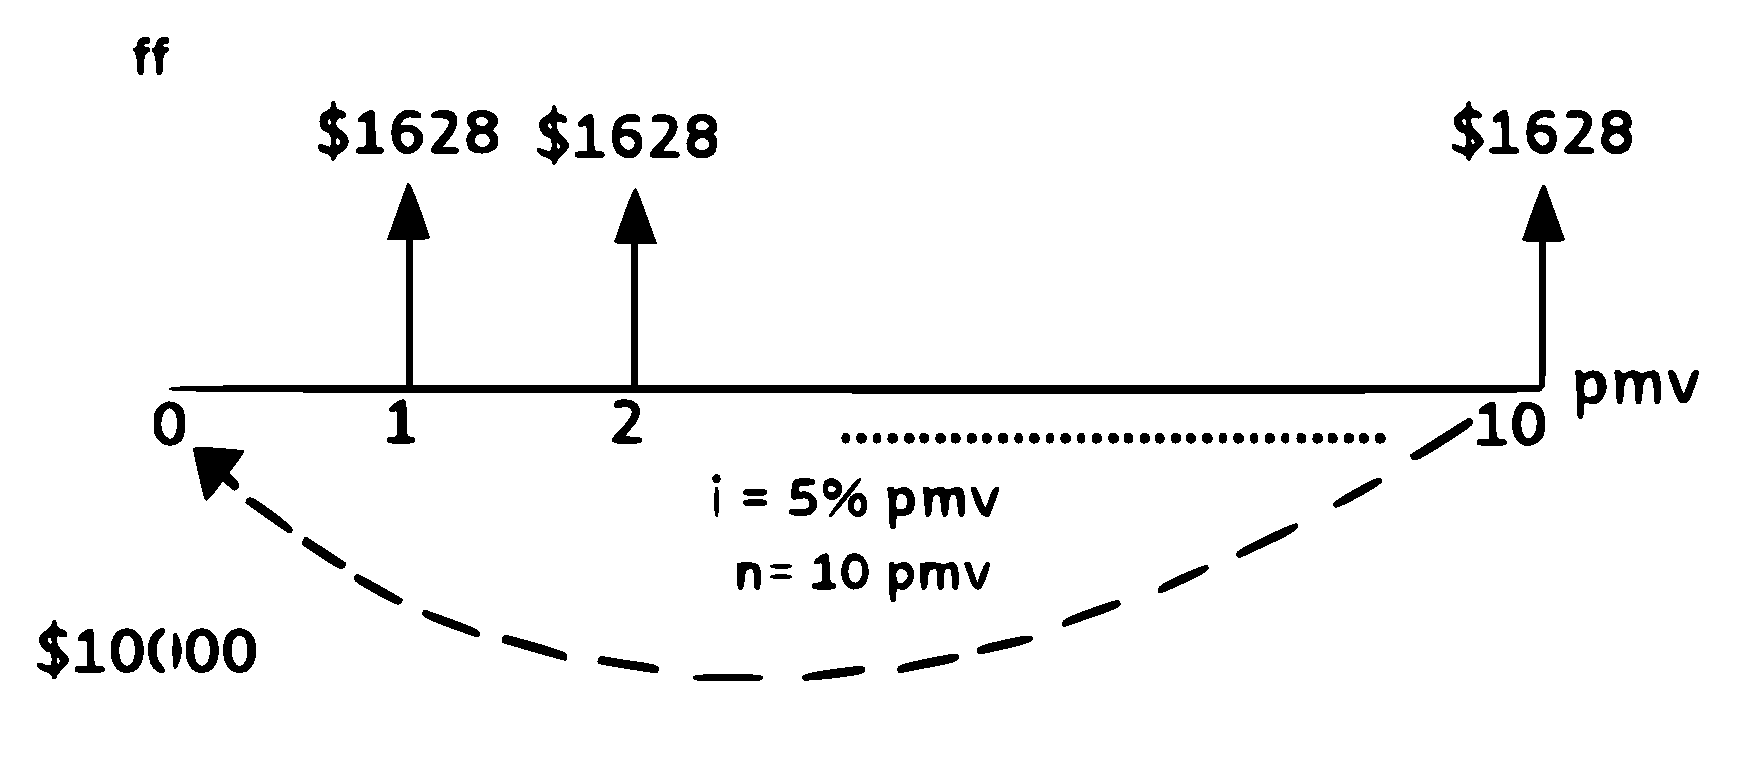
\includegraphics[scale=0.4, trim=-5 -5 -5 -5]{Graf9Cap11.pdf} }  
   \\\hline
		%%%%%%%%%%%%% FIN INSERCIÓN DE IMAGEN
		%%%%%FIN FLUJO DE CAJA
		
		
		
		%%%%% INICIO DECLARACIÓN FORMULAS
		%%%%%%%%%%% INICIO TITULO
\rowcolor[HTML]{FFB183}
\multicolumn{3}{|c|}{\cellcolor[HTML]{FFB183}\textbf{4. Declaración de fórmulas}}    \\ \hline
		%%%%%%%%%%% FIN TITULO
		%%%%%%%%%%% INICIO MATEMÁTICAS
\multicolumn{3}{|c|} {VPN =	$\sum F_{n}(1+i)^{-n}$   Valor presente neto.}   \\ \hline	
	
		%%%%%%%%%% FIN MATEMÁTICAS
		%%%%%% INICIO DESARROLLO MATEMÁTICO
\rowcolor[HTML]{FFB183}
		%%%%%%%%%%INICIO TITULO
\multicolumn{3}{|c|}{\cellcolor[HTML]{FFB183}\textbf{5. Desarrollo matemático}}       \\ \hline
		%%%%%%%%%% FIN TITULO
		%%%%%%%%%% INICIO MATEMÁTICAS
		\multicolumn{3}{|c|}{$ VPN(A)=-  COP  200.000+  COP  31.160(\frac{1-(1+0.05)^{-10}}{0.05})=  COP  40.609,26 $}  
		\\
		
		\multicolumn{3}{|c|}{$ VPN(B)=-  COP  100.000+  COP  16.280(\frac{1-(1+0.05)^{-10}}{0.05})=  COP  25.709,84 $}  
		\\
		\multicolumn{3}{|c|}{$ \textbf{El VPN nos dice que es mejor el proyecto A}$}  
		\\
		\multicolumn{3}{|c|}{$ \textbf{Evaluando el TIR}$}  
		\\
		\multicolumn{3}{|c|}{$ TIR(A)=  COP  200.000+  COP  31.160(\frac{1-(1+i)^{-10}}{0.05})=  COP  0 $}  
		\\
		\multicolumn{3}{|c|}{$ \text{Calculando i por interpolación se tiene que i=9\% pmv} $}  
		\\
		\multicolumn{3}{|c|}{$ TIR(B)=-  COP  100.000+  COP  16.280(\frac{1-(1+i)^{-10}}{0.05})=  COP  0 $}  
		\\
		\multicolumn{3}{|c|}{$ \text{Calculando i por interpolación se tiene que i=10.01\% pmv} $}  
		\\
		\multicolumn{3}{|c|}{$ \text{La TIR nos dice que es mejor el proyecto B, lo cual contradice al VPN.} $}  
		\\
		\multicolumn{3}{|c|}{$ \text{Intentamos aclarar esta contradicción usando la TIRM.} $}  
		\\
		\multicolumn{3}{|c|}{$ \textbf{Evaluando la TIRM } $}  
		\\
		\multicolumn{3}{|c|}{$ \text{TIRM(A):  Trasladamos a valor final la serie de 10 ingresos de  COP  31.160 y tenemos:} $}  
		\\
		\multicolumn{3}{|c|}{$ COP  31.160(\frac{(1+0.05)^{10}-1}{0.05})=  COP  391.927,13  \textbf{ Ecuación de valor }$}  
		\\
		\multicolumn{3}{|c|}{ 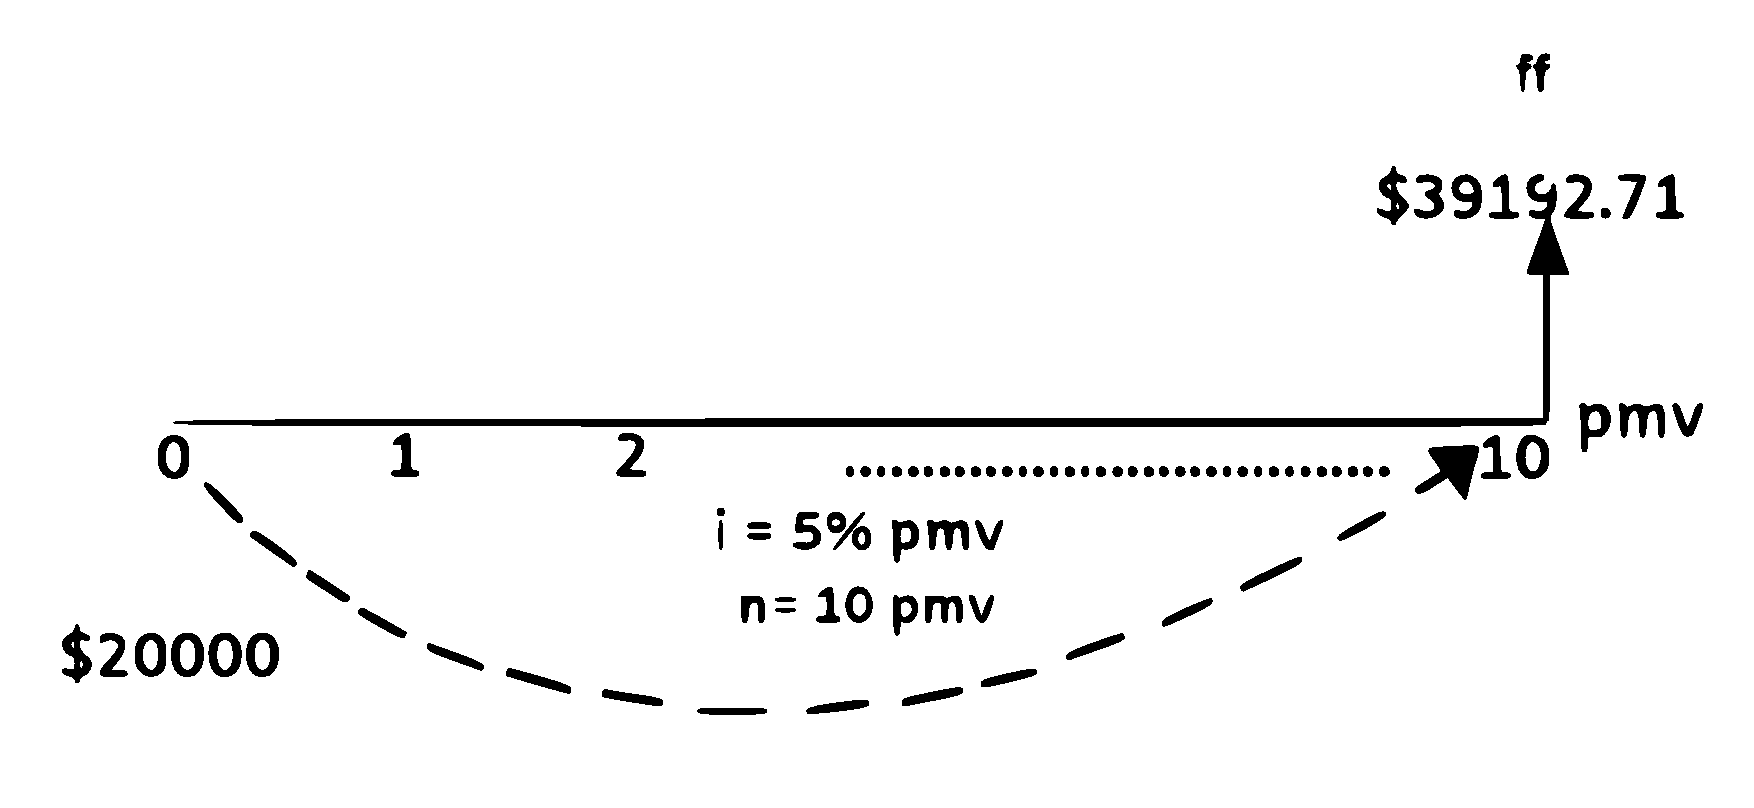
\includegraphics[scale=0.4, trim=-5 -5 -5 -5]{Graf10Cap11.pdf} }   
		\\ 
		\multicolumn{3}{|c|}{$ COP  391.927,13=  COP  200.000(1+i)^{10}$}  
		\\
		\multicolumn{3}{|c|}{$TIRM(A)= i= 6.96\% pmv$}
		\\
		\multicolumn{3}{|c|}{$ \text{TIRM(B):  Trasladamos a valor final la serie de 10 ingresos de  COP  16.280 y tenemos:} $}  
		\\
		\multicolumn{3}{|c|}{$  COP  16.280(\frac{(1+0.05)^{10}-1}{0.05})=  COP  204.768,1  \textbf{    Ecuación de valor }$}  
		\\
		\multicolumn{3}{|c|}{ 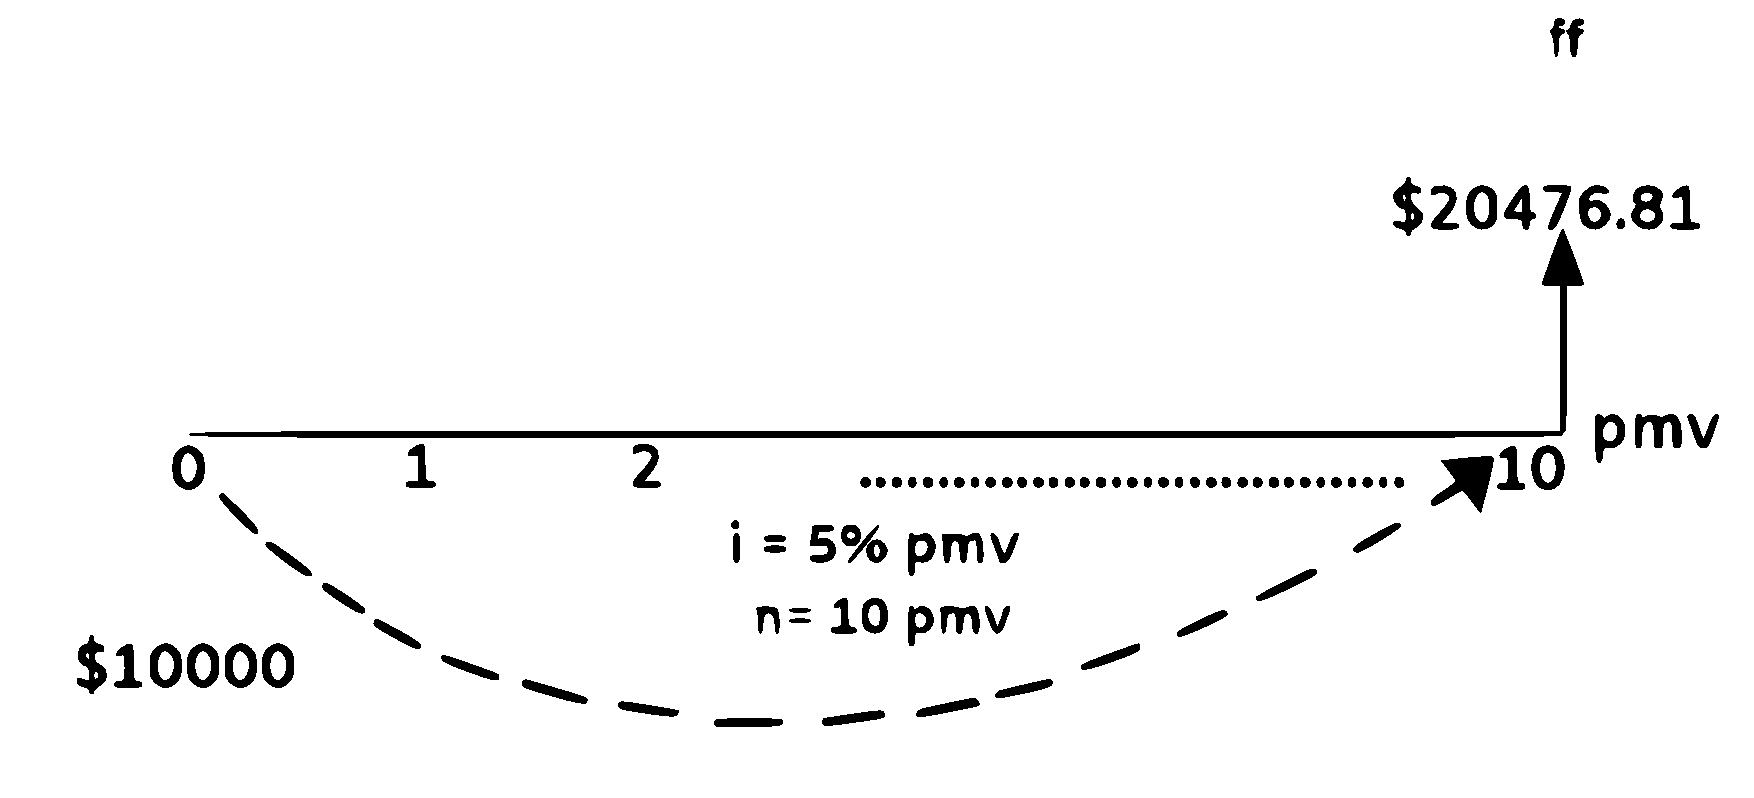
\includegraphics[scale=0.4, trim=-5 -5 -5 -5]{Graf11Cap11.pdf} }   
		\\ 
		\multicolumn{3}{|c|}{$ COP  204.768,1=  COP  10.000(1+i)^{10}$}  
		\\
		\multicolumn{3}{|c|}{$TIRM(B)= i= 7.43\% pmv$}
		\\
		\multicolumn{3}{|c|}{$\text{Se concluye que TIRM(B) es mejor que TIRM(A)}$}
		\\
		\multicolumn{3}{|c|}{$\text{Como el proyecto A es más costoso que el proyecto B debemos adicionar al proyecto B   }$}
		\\ 
		\multicolumn{3}{|c|}{$\text{el proyecto adicional con inversión inicial de  COP  100.000 y lo evaluaremos a la tasa del 5\% pmv.  }$}
		\\ 		
		\multicolumn{3}{|c|}{$  COP  100.000(1+0.05)^{10}=  COP  162.889,46$}
		\\ 	
		\multicolumn{3}{|c|}{ 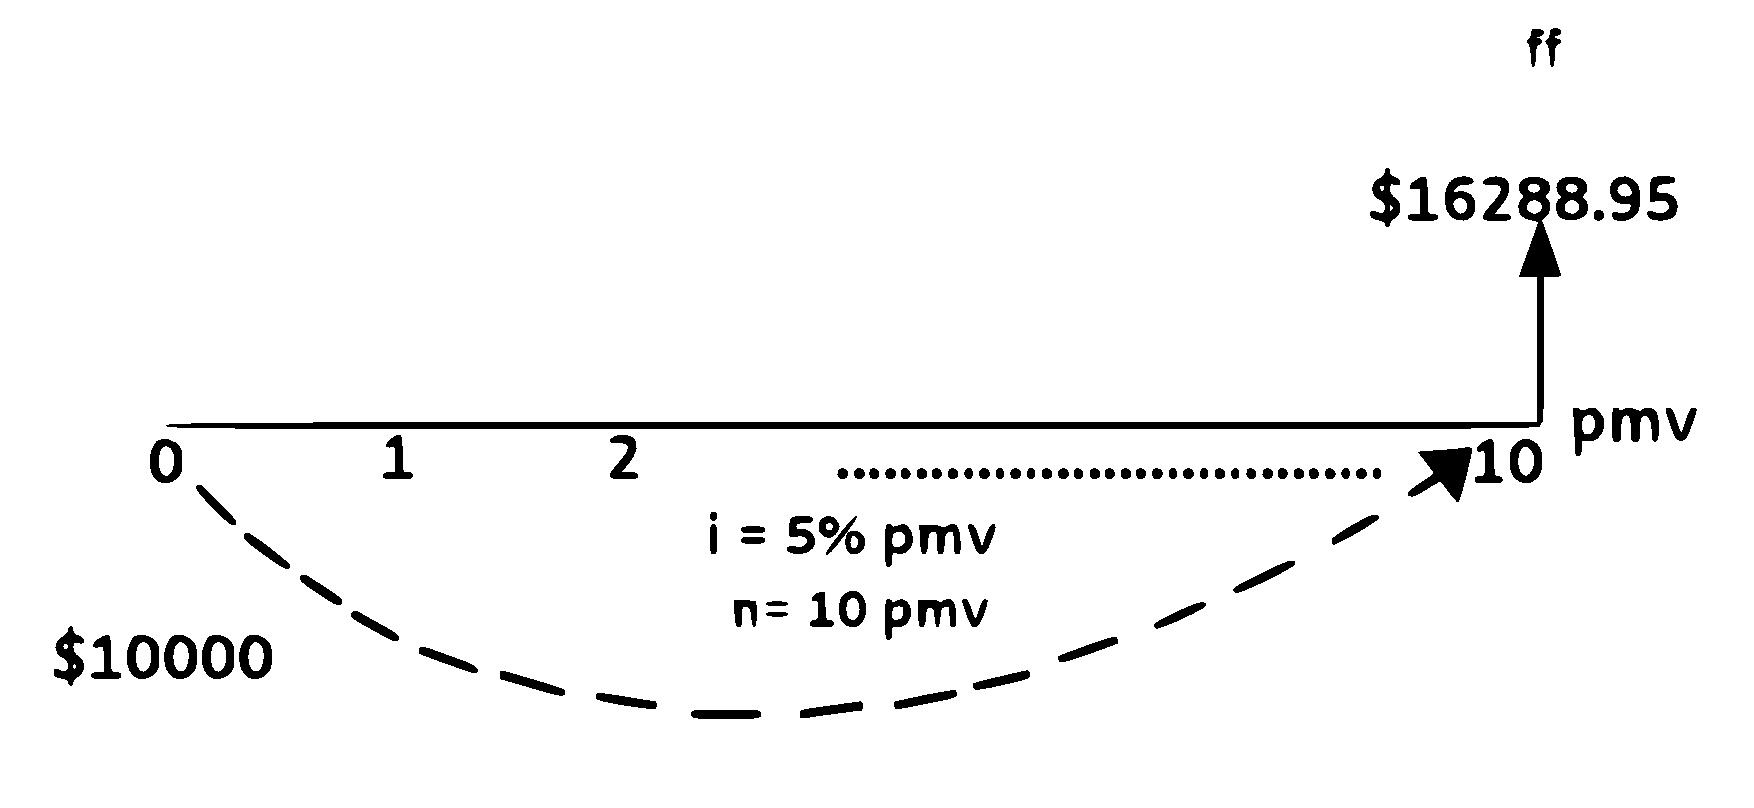
\includegraphics[scale=0.4, trim=-5 -5 -5 -5]{Graf12Cap11.pdf} }   
		\\ 
		\multicolumn{3}{|c|}{$\text{Entonces el nuevo proyecto B quedará formado por el proyecto B incial   }$}
		\\ 
		\multicolumn{3}{|c|}{$\text{más el proyecto adicional con el siguiente flujo de caja:  }$}
		\\ 
		\multicolumn{3}{|c|}{$\textbf{Ingresos en el periodo 10: }  COP  204.768,1+  COP  162.889,46=  COP  367.657.56 $}
		\\ 
		\multicolumn{3}{|c|}{$\textbf{Costo inicial: }  COP  100.000+  COP  100.000=  COP  200.000$}
		\\
		\multicolumn{3}{|c|}{ 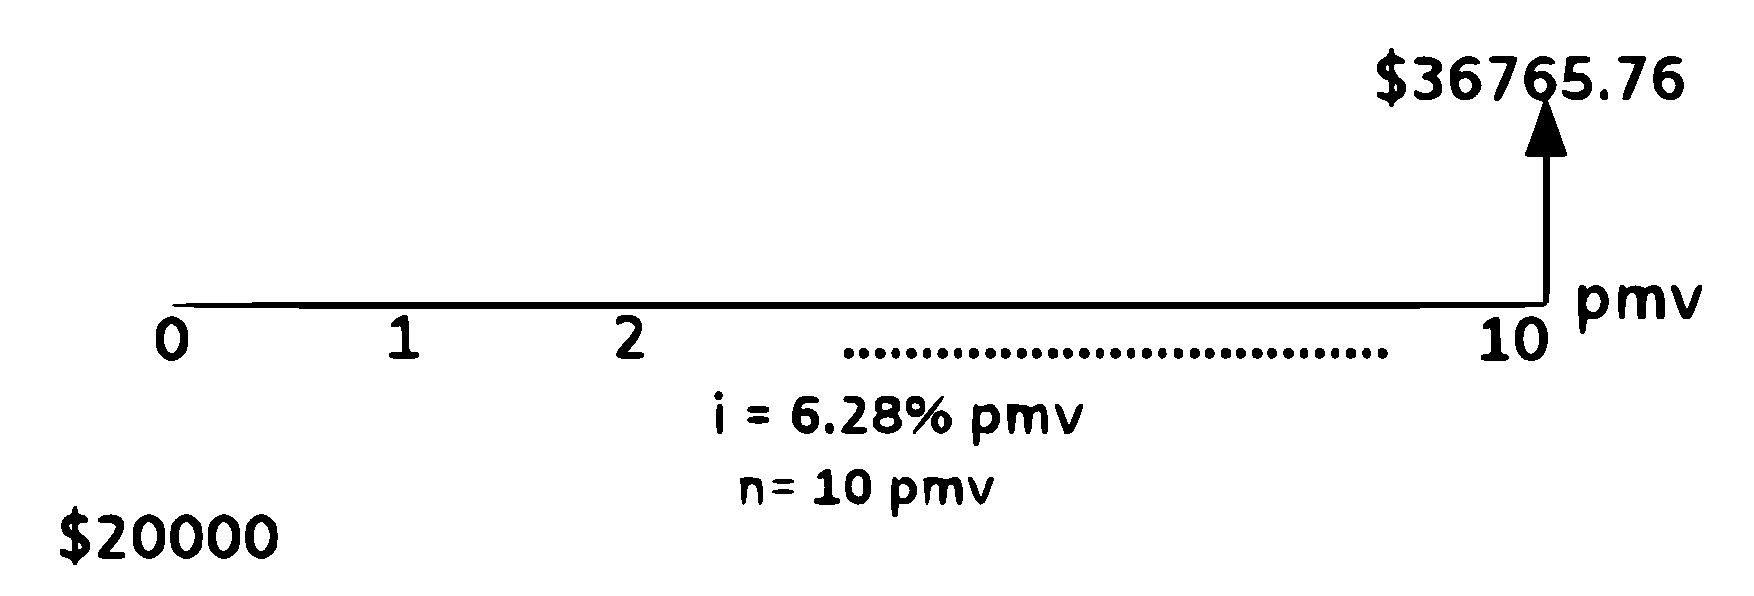
\includegraphics[scale=0.4, trim=-5 -5 -5 -5]{Graf13Cap11.pdf} }   
		\\ 
		\multicolumn{3}{|c|}{$\text{ Ahora calculamos la TIR de este nuevo proyecto así: } $}
		\\
		\multicolumn{3}{|c|}{$ COP  367.657,56=  COP  200.000(1+i)^{10}$}
		\\
	    \hline
				
		%%%%%%%%%% FIN MATEMÁTICAS
		%%%%%% FIN DESARROLLO MATEMÁTICO
		%%%%%% INICIO RESPUESTA
\rowcolor[HTML]{FFB183}
		%%%%%%%%%%INICIO TITULO
\multicolumn{3}{|c|}{\cellcolor[HTML]{FFB183}\textbf{6. Respuesta}}   \\ \hline
		%%%%%%%%%% FIN TITULO
		%%%%%%%%%% INICIO RESPUESTA MATEMÁTICA
		
\multicolumn{3}{|c|}{ \text{Al despejar se tiene que i=6.28\% pmv el cual es inferior a la TIR del proyecto A}}
\\
\multicolumn{3}{|c|}{\text{y el ordenamiento que produce la TIR coincide con el ordenamiento que produce el VPN. } }
\\
\hline

		
		%%%%%%%%%% FIN MATEMÁTICAS
		%%%%%% FIN RESPUESTA
	\end{longtable}
	%Se crean dos lineas en blanco para que no quede el siguiente texto tan pegado
	%\newline \newline %USARLO SI CREES QUE ES NECESARIO
\end{center}
%%%%%%%%%%%%%%%%%%%%%%%%%%FIN EJERCICIO 1 %%%%%%%%%%%%%%%%%%%%%%%%%%%


\textbf{}\\
